\subsection{Análisis}

Durante la etapa de análisis del primer incremento se llevó a cabo una investigación para seleccionar las tecnologías y herramientas que se utilizarían para el desarrollo del proyecto. Además, se recopilaron aquellos requisitos funcionales y no funcionales relacionados con la autenticación del usuario y gestión de cuentas. Finalmente, se elaboró un diagrama de casos de uso que que servirá como representación visual de las funcionalidades implementadas.

Con respecto a la investigación de tecnologías y herramientas, se seleccionaron las siguientes:

\begin{itemize}
    \item \textbf{\textit{Next.js}} como \textit{framework fullstack}, debido a su popularidad en el desarrollo de aplicaciones web y la amplia disponibilidad de referencias y documentación.
    \item \textbf{\textit{Tailwind CSS}} como \textit{framework} de estilos, por la capacidad que ofrece al desarrollador para definir estilo de forma rapida y eficaz.
    \item \textbf{\textit{Vitest}} como \textit{framework} de pruebas unitarias, ofreciendo las herramientas necesarias para la ejecución de pruebas utilizando \textit{\gls{mock}}.
    \item \textbf{\textit{Supabase}} como plataforma \textit{back-end}, por su amplio catalogo de funcionalidades desde creación y gestión de tablas, autenticación de usuarios y ejecución de procesos automatizados a través de \textit{triggers} y funciones.
\end{itemize}

Se seleccionaron los siguientes requisitos funcionales y no funcionales relacionados con la \textbf{implementación de registro, autenticación y perfil de usuario}, \tabref{tab:requisitosfuncionalesincremento1} y \tabref{tab:requisitosnofuncionales}.

\begin{table}[H]
    \centering
    \scriptsize
    \begin{tabular}{l p{0.58\textwidth} p{0.20\textwidth} l}
        \textbf{ID} & \textbf{Requisito Funcional} & \textbf{Funcionalidad} & \textbf{Prioridad} \\ \hline
        RF1  & El usuario debe poder iniciar y cerrar sesión. & Cuenta de usuario & Alta \\ \hline
        RF2  & El usuario debe poder registrarse utilizando su correo electrónico, contraseña y un nombre de usuario. & Cuenta de usuario & Alta \\ \hline
        RF3  & El usuario debe poder modificar su perfil. & Cuenta de usuario & Alta \\ \hline
        RF4  & El usuario debe poder eliminar su cuenta. & Cuenta de usuario & Alta \\ \hline
        RF5  & El usuario debe poder recuperar o restablecer su contraseña en caso de olvido. & Cuenta de usuario & Alta \\ \hline
    \end{tabular}
    \caption{Requisitos Funcionales desarrollados en el incremento 1}\label{tab:requisitosfuncionalesincremento1a}
\end{table}

\begin{table}[H]
    \centering
    \scriptsize
    \begin{tabular}{l p{0.79\textwidth} l}
    \textbf{ID} & \textbf{Requisito No Funcional} & \textbf{Prioridad} \\ \hline
    RNF1 & El sistema debe ser responsivo, adaptándose a diferentes tamaños de pantalla y dispositivos. & Alta \\ \hline
    RNF2 & El sistema debe incluir una descripción textual (alt) en todas las imágenes. & Alta \\ \hline
    RNF3 & El sistema debe incluir un aria-label o aria-labelledby en todos los elementos interactivos, describiendo su función para lectores de pantalla. & Alta \\ \hline
    RNF4 & El sistema debe proporcionar navegación mediante un encabezado (header) y un pie de página (footer) consistentes en todas las vistas. & Alta \\
    \end{tabular}
    \caption{Requisitos No Funcionales desarrollados en el incremento 1}\label{tab:requisitosnofuncionalesa}
\end{table}

Finalmente, tomando como referencia los requisitos seleccionados, se elaboró un diagrama de casos de uso:

\begin{figure}[H]
    \centering
    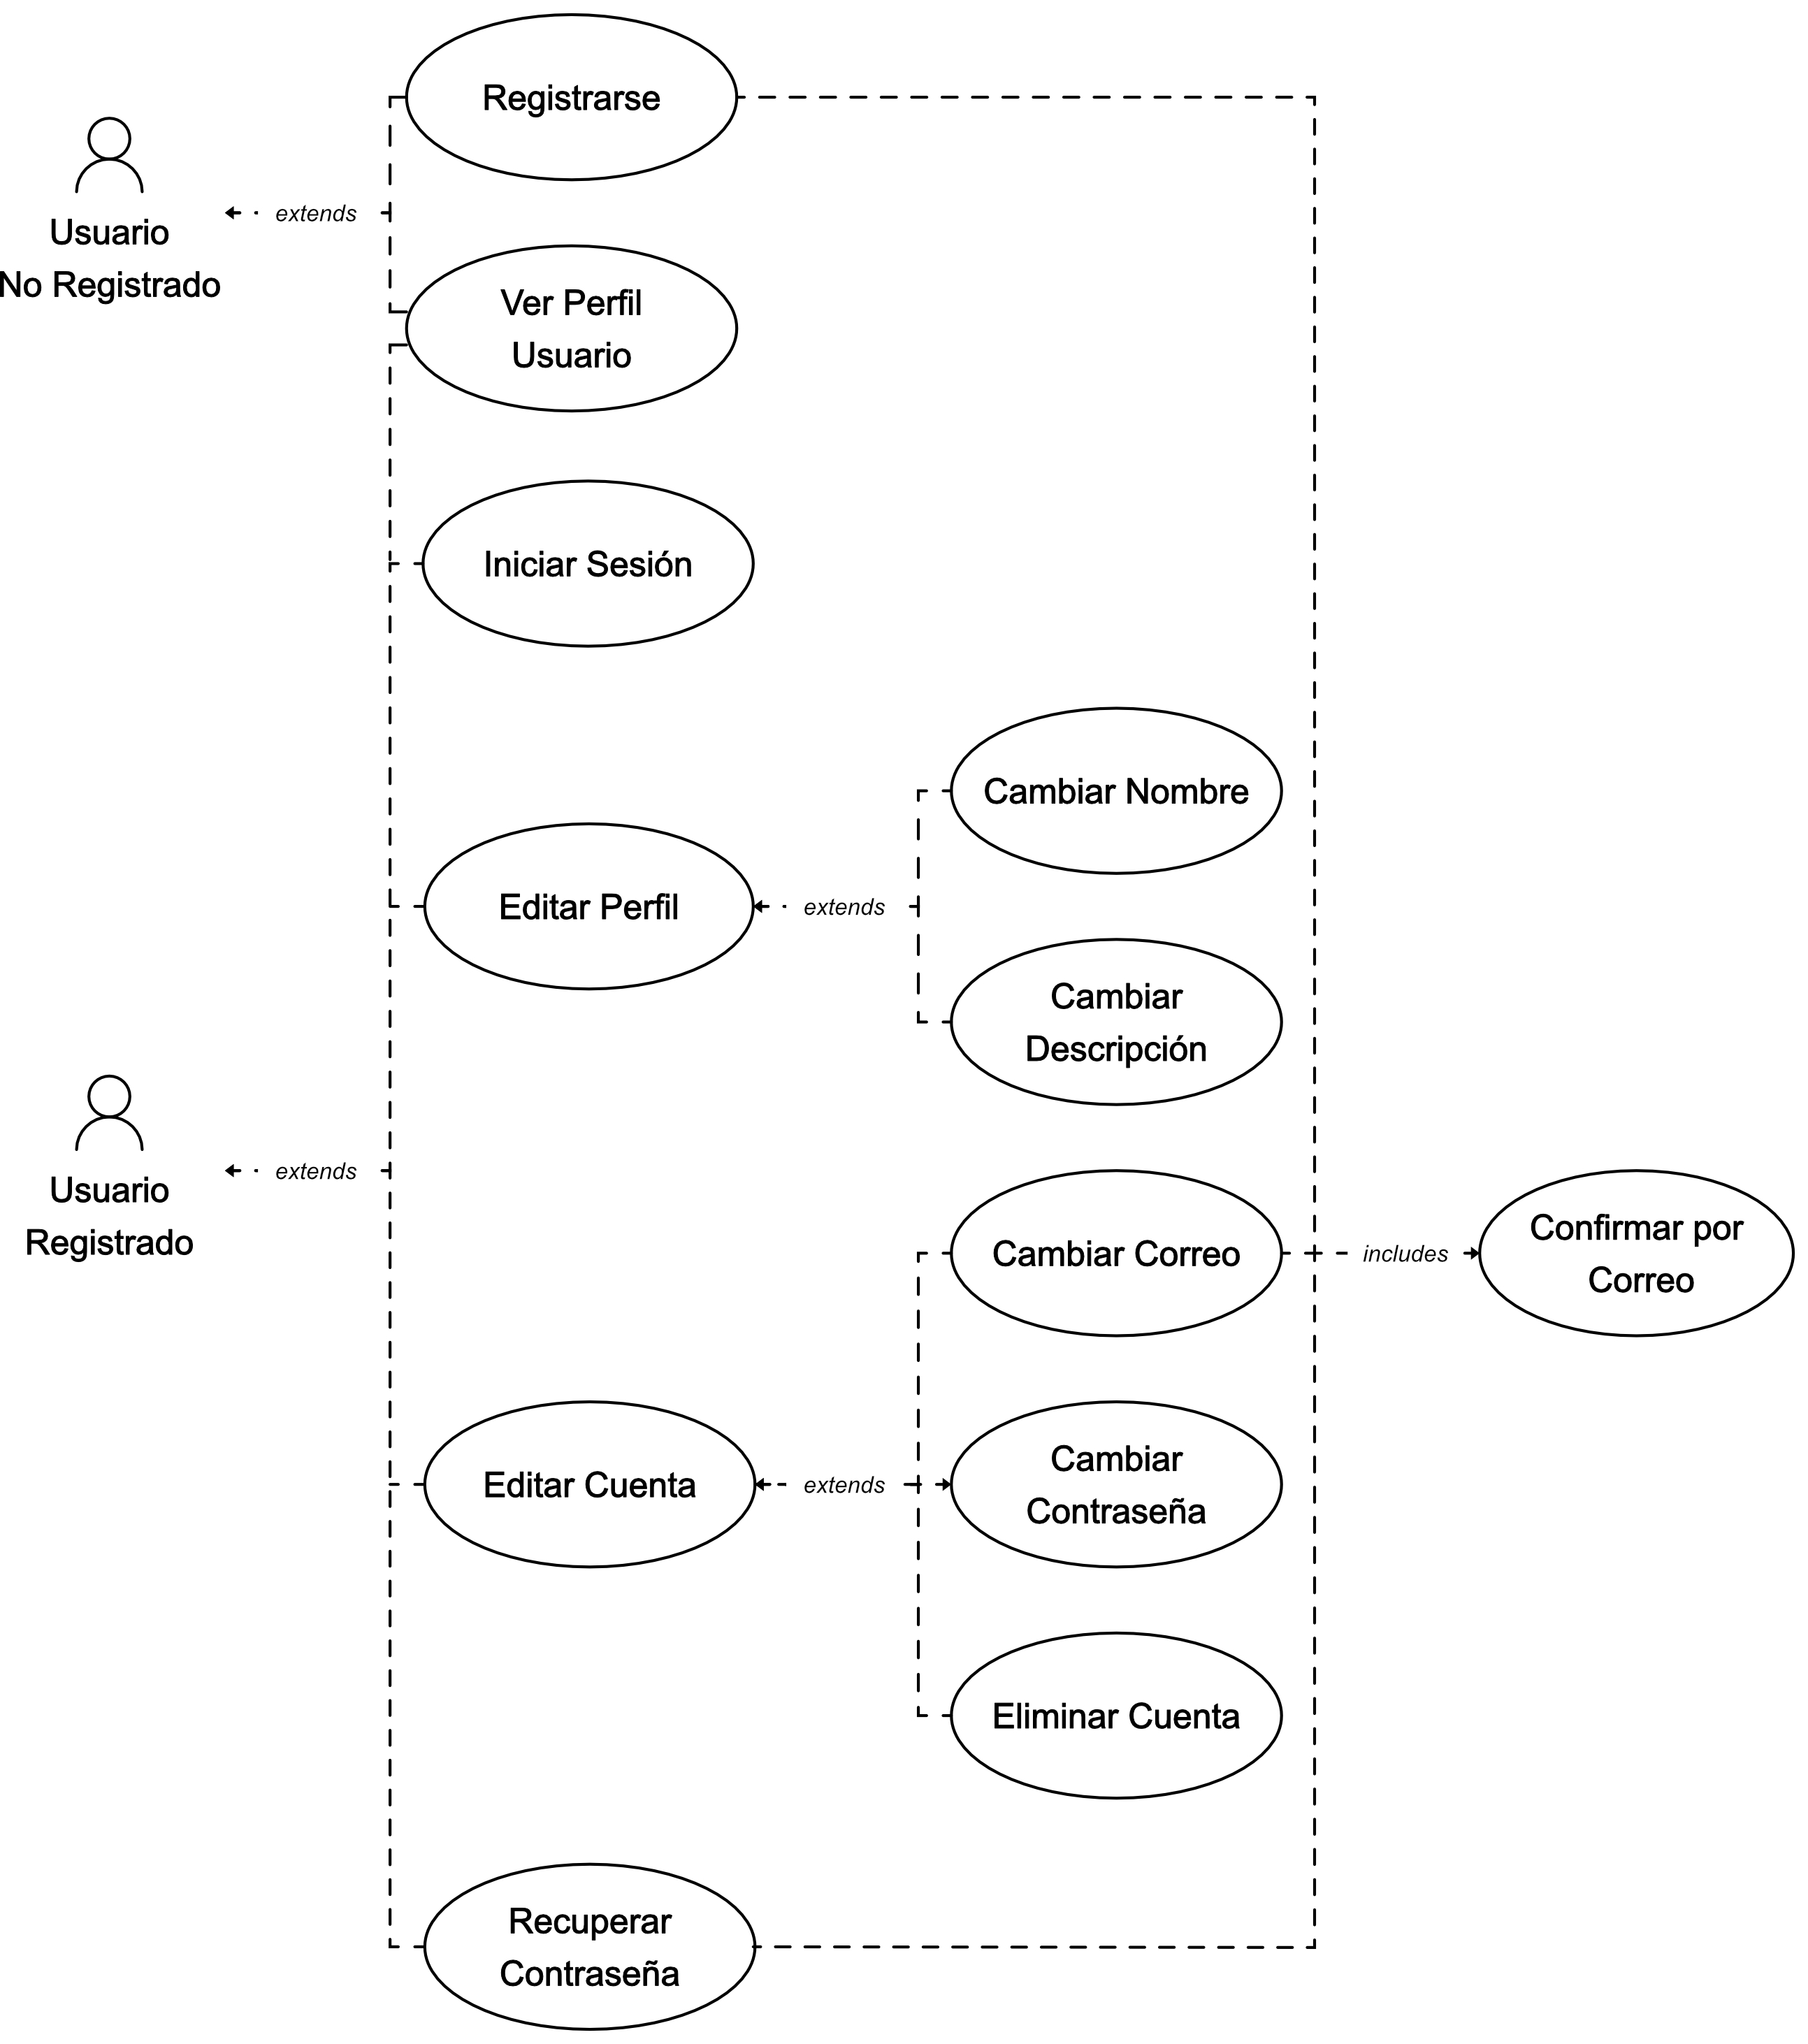
\includegraphics[width=0.5\textwidth]{Ilustraciones/desarrollo/incremento1/analisis/cu_i1.jpg}
    \caption{Casos de uso del incremento 1}\label{fig:cu_i1}
\end{figure}
